%%%%%
%%Title: HiPi+Bus V0.2 Chapter 6
%%Creator: Ando Ki
%%CreationDate: April 1992
%%FileName: sec4
%%RelatedFile: ch6
%%%%%
\section{데이터 전송버스의 시간규격}
데이터 전송 버스는 동기형 제어 방식을 사용함에 따라 모든 신호는 한개 클럭 주기 동안에 버스 상에서
구동되고 감지하게 된다. 따라서 모든 신호는 데이터 전송 프로토콜에서 규정된대로
자신에게 할당된 주기에 언제나 한개 버스 클럭 동안만 구동을 하게된다.
%
%\documentstyle[a4]{hbook}
%\begin{document}
%
\begin{table}[htbp]
\caption{데이터 전송 버스 신호의 시간규격 요약}\label{table:dtb-time}
   \begin{center}
   \begin{tabular}{|l|l|r|r|r|} \hline
	timing parameter & name & min & typical & max \\ \hline \hline
	$TP^{BCLK}_0$ & BCLK* cycle time & 59 & 60 & 61 \\ \hline
	$TP^{DTB}_0$  & DTB signal latch point & 38 & 40 & 42 \\ \hline
	$TP^{DTB}_1$  & bus propagation time & - & - & 20 \\ \hline
	$TP^{DTB}_2$  & setup time & 10 & - & - \\ \hline
	$TP^{DTB}_3$  & hold time & 5 & - & - \\ \hline
	$TP^{DTB}_4$  & guard time & 10 & - & - \\ \hline
   \end{tabular}
   \end{center}
\end{table}
%
%\end{document}

\begin{figure}[htb]
    \centerline{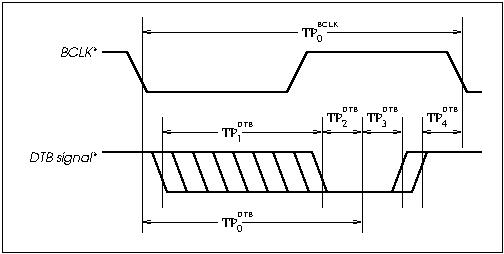
\includegraphics{ch6/FIG/dtb-time.jpg}}
   \caption{데이터 전송버스 신호의 시간규격}\label{figure:dtb-time}
\end{figure}
%

데이터 전송버스의 모든 정보는 백플레인에 나타나는 버스클럭 신호의 하강점으로부터
$TP^{DTB}_0$(DTB signal latch time)후에
데이터 전송버스 정보를 안정되게 래치할 수 있도록 보장해야 한다.
이를 위하여 셋업시간(setup time)으로 $TP^{DTB}_2$를
홀드시간(hold time)으로 $TP^{DTB}_3$를 반드시 보장해야 한다.
그리고 이어지는 버스클럭에 구동될 신호와의 충돌을 방지하기 위해
$TP^{DTB}_4$를 보장해야 한다.
%
%%%%%
